% Your name
\renewcommand{\YRname}{R. Oechslin}

% Your grade/post
\newcommand{\YRgrade}{M2}

% Submission date
\newcommand{\YRdate}{2018.Jul.31}

% Your research theme
\newcommand{\YRtheme}{Haptic Feedback Controller with Palm Pressurization}

% Work plan
\newcommand{\YRplan}{
	\hspace{-4truemm}
	\begin{tabularx}{170truemm}{|p{50truemm}||X|X|X|X|X|X|X|X|X|X|X|X|}
		\hline
		\multicolumn{13}{|c|}{\parbox[c][10truemm][c]{0truemm}{} \large Research theme: \bf \YRtheme} \\
		\hline
		\hline
		\multicolumn{13}{|c|}{\parbox[c][8truemm][c]{0truemm}{} \large \bf --- Research Plan ---} \\
		\hline
		Term \textbackslash Month & 2 & 3 & 4 & 5 & 6 & 7 & 8 & 9 & 10 & 11 & 12 & 1 \\
		\hline
		% For ``Work plan'', do not change above.
		\hline
		Literature review & & & & & & & & & & & & \\
		\shadecells{2-2}
		\hline
		Design PlayStation Controller  & & & & & & & & & & & & \\
		\shadecells{2-3}
		\hline
		Test PlayStation Controller & & & & & & & & & & & & \\
		\shadecells{4-6}
		\hline
		Frequency Response Analysis & & & & & & & & & & & & \\
		\shadecells{5-6}
		\hline
		Design Pilot Controller & & & & & & & & & & & & \\
		\shadecells{4-6}
		\hline
		Test Pilot Controller & & & & & & & & & & & & \\
		\shadecells{6-7}
		\hline
		& & & & & & & & & & & & \\
		%\shadecells{2-10}
		\hline
		Theoretical Analysis & & & & & & & & & & & & \\
		\shadecells{6-7}
		\hline
		Analyze data and compare & & & & & & & & & & & & \\
		\shadecells{7-8}
		\hline
		Write Thesis & & & & & & & & & & & & \\
		\shadecells{8-8}
		\hline
	\end{tabularx}
}

% Main contents of your work
\newcommand{\YRachievement}{
	
\section{Introduction}
This report is the continuation of the first two reports about the project "Haptic Feedback Controller with Palm Pressurization". The last report has stated the tracking behavior of a simple P- and PID-controlled device for a sine reference of various frequencies. Furthermore, it has suggested an experimentally identified equivalent spring damping coefficient which can be used to model the setup analytically.\\
This report is first introducing a thorough literature research into the haptic teleoperated field of study. Then it will discuss the results of the tested controller and give advice on how to choose system and setup parameters for future and related work. 

\section{Project Introduction}
\subsection{Haptics}
The Oxford Dictionaries defines haptics as 

%\begin{displayquote}
"Relating to the sense of touch, in particular relating to the perception and manipulation of objects using the senses of touch and proprioception." \cite{Oxford}
%\end{displayquote}
It dates the term back to the late 19th century	and states its origin from the greek words \textit{haptikos} meaning 'able to touch or grasp' and \textit{haptein}, 'fasten'.\\
In engineering, the research in the haptic field has started to emerge in late nineteen-eighties \cite{Srinivasan1995}. Before that, man-machine interaction was mainly limited to keyboard and mouse input, which is rather unidirectional and passive and it soon has become clear that this requires a more skilled user for all kinds of operations. This directly leads to limitations in performance. Haptics can extend this unilateral interaction by providing tactile or kinesthetic information. This combination can overcome the users limitations and improve performances of high-precision tasks or high-force tasks drastically.\\
\cite{Hayward2004} states, that even though the research in the haptic domain in the past ten years has significantly increased, further investigations are necessary for the "quest for realism", especially in medical telesurgical applications where realism is key to performance. Other application domains include space operations, manufacturing, physical rehabilitation, arts or simply entertainment related devices.\\
\cite{Adams1998} states the critical elements for stability of haptic setups, mainly focusing on haptic simulations. It also motivates exploration of alternative control techniques due to the unpredictability of the human operator and the environment model.
%why haptics and what is it, needs identification

%TODO stated already in april \subsection{Previous Research at Yamamoto's Lab}
%what are the problems of the research before i came
%TODO stated already in april \subsection{Literature Review}
%what are some similar applications
%TODO stated already in april \subsection{Project Scope}
%what are my goals



%	\begin{figure}[h!]
%		\centering
%		\begin{tabular}{|l|c|c|}%designator | explanation | unit
%			\hline
%			 Designator & Explanation & Unit \\ \hline \hline
%			$T_m$ & Motor torque & [Nm]\\ 
%			$T$ & Output torque acting on carriage& [Nm]\\
%			$b_{op}$ & Damping coefficient of the operator & [Ns/m]\\
%			$J_T$ & Total inertia of mechanical setup & [$\textit{kgm}^2$]\\
%			\hline
%		\end{tabular}
%		\caption{Setup parameters}
%		\label{tab:setup_params}
%	\end{figure}

\section{Stability and Transparency Trade-Off}
Even though the controller cannot be seen as a master-slave teleoperation setup, the problem settings of stability and transparency still apply. They are the main problems related to haptics and haptic teleoperation applications \cite{Christiansson2007}. Often, the stability issues arise from master-slave mass mismatch and stiffness of the environment. But high inertia also poses problems for higher frequencies. In this research however, the masses and frequencies are relatively low. \\
The stability of this controller is not only affected by the control scheme and the mechanical setup, but also by the operator, whose grasp can render a system stable or unstable \cite{Enayati2016}. Additionally, communication delays can also cause instability.\\
To gain insight into the stability, literature uses for example the root-locus method \cite{Christiansson2006} or the notion of passivity. For haptics, it can generally be assumed that the operator is passive \cite{Hogan1989}. Alternatively, one can also use the real data of the implementation to subjectively assess the stability. Here, the latter approach has been chosen.

%Hannaford shows that a cable driven hand-controller has similar frequency characteristics, where the resonance frequency is slightly more elevated than the SEA device.

\section{PlayStation-Controller Testing}
\begin{figure}[h!]
	\centering
	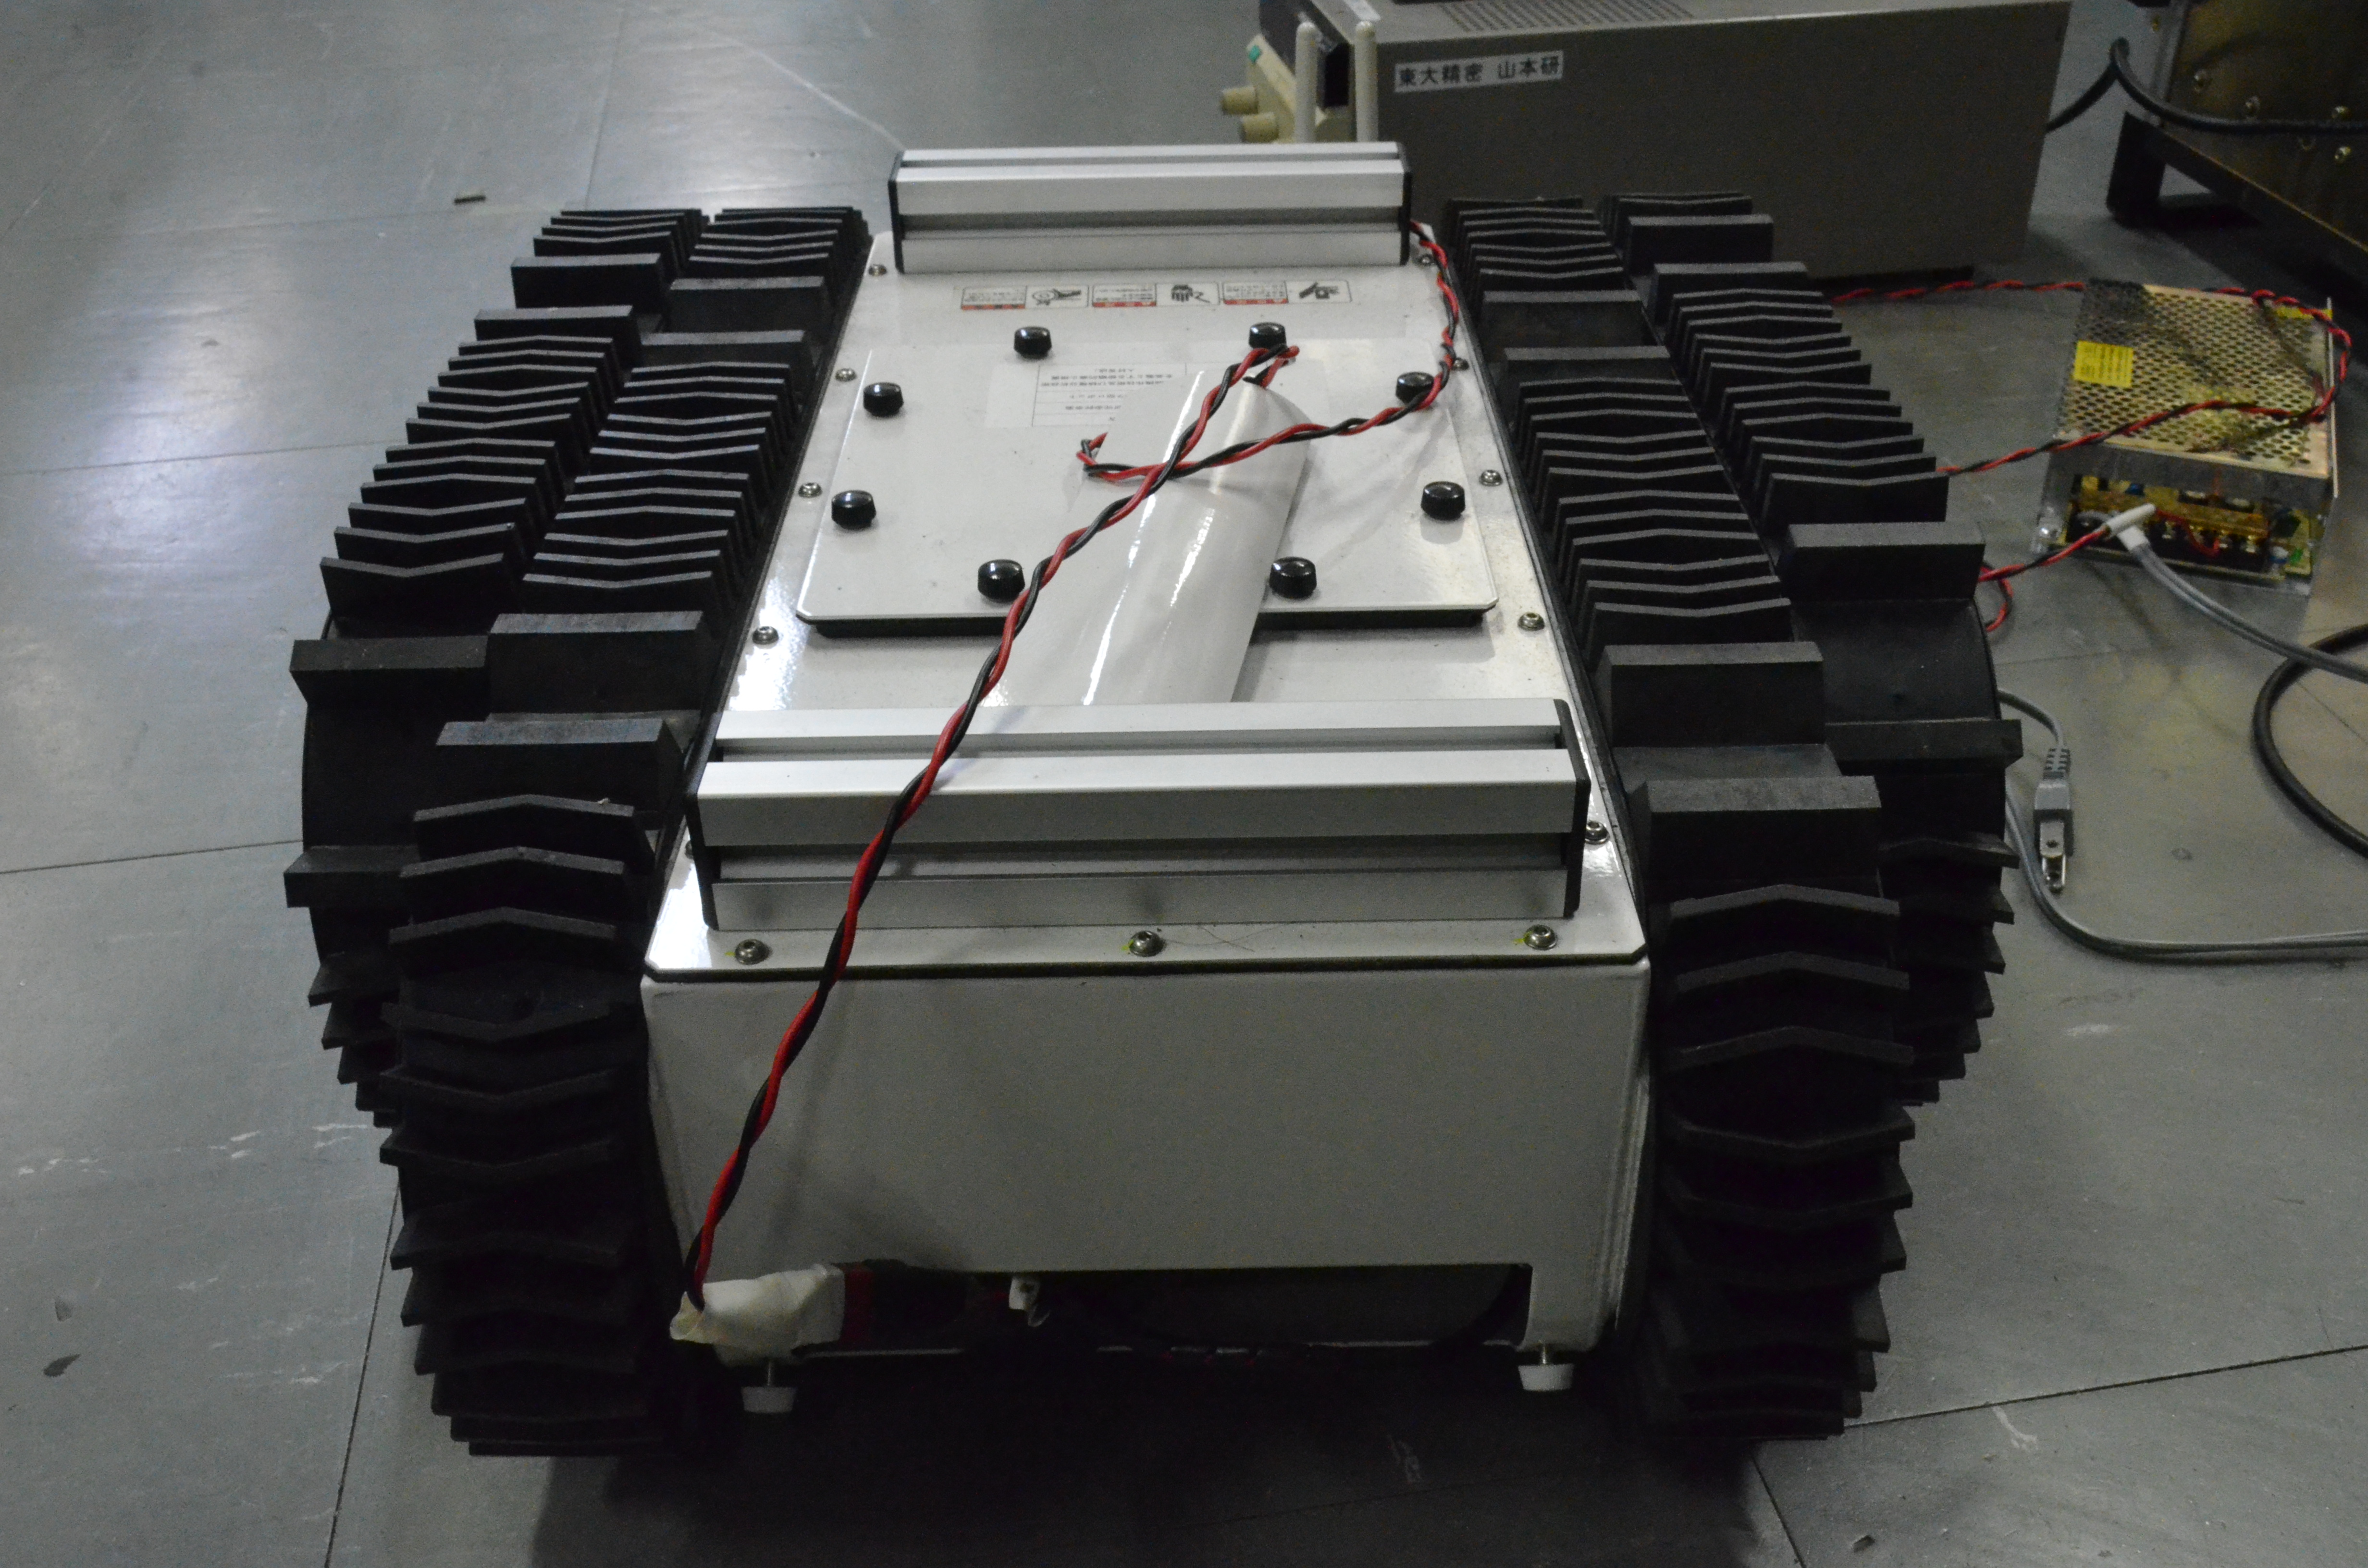
\includegraphics[width=0.6\linewidth]{Figs/topy_robot}
	\caption{Topy robot for real-world controller test setup.}
	\label{fig:topy_robot}
\end{figure}
After the theoretical analysis and model identification of the PlayStation-controller, the setup has been put to the test. At first, the controller has been connected to the computer to communicate with the Topy robot. The communication software was written in processing \cite{Fry2018} and is explained in a different section.\\ %TODO write about the software somewhere, reference here
\subsection{Latency}
The controller was successfully able to navigate the robot, if with a delay of roughly $700$ms. The commercial controller, that was developed for the Topy robot, also had a certain delay of almost $500$ms. This delay is the difference between the instant when the joystick is pushed forward, and the moment when the robot starts moving. The feedback methods that have been tested varied between a pure pitch feedback, a combined pitch and roll feedback and a current consumption feedback law. \\%TODO state the feedback laws and reference here
The effect and magnitude of the command latency, but also of the feedback latency can be seen in figure \ref{fig:real_P_scope_13_latency_plot} and \ref{fig:real_PID_scope_14_latency_plot}.

\begin{figure}[h!]
	\centering
	\includegraphics[width=1\linewidth]{Figs/real_P_scope_13_latency_plot}
	\caption{Command and behavior of Topy robot with P-controlled PlayStation controller.}
	\label{fig:real_P_scope_13_latency_plot}
\end{figure}


\begin{figure}[h!]
	\centering
	\includegraphics[width=1\linewidth]{Figs/real_PID_scope_14_latency_plot}
	\caption{Command and behavior of Topy robot with PID-controlled PlayStation controller.}
	\label{fig:real_PID_scope_14_latency_plot}
\end{figure}

In these figures, several interesting things have to be mentioned. First of all, the delay between sending the commands and receiving the consumed current value, which is then used as feedback value, is roughly $700$ ms. The delay between the received feedback value and the response of the distance sensor is much smaller and depends on the situation of the robot. When the robot starts to move, it takes some time until the current has built up, and the latency between the reference compression and actual compression is roughly $130$ ms for the P-controlled, and $430$ ms for the PID-controlled setup (see first red vertical lines). However, when the robot is stopped, the latency is $20$ - $30$ ms (second and third red lines).\\
In the first green lines, an external force has been applied to the robot, simulating an obstacle, which increased the consumed current and therefore also increased the desired feedback value. Again, the latency was of roughly $30$ ms. The second green lines is where the external force has been removed and the current dropped abruptly back to its normal value. The latency here was below $10$ ms.\\
Also indicated in figures \ref{fig:real_P_scope_13_latency_plot} and \ref{fig:real_PID_scope_14_latency_plot}, one can see that the feedback has been turned off when driving backwards (balck lines). However, in this scenario the feedback has been activated when standing still, ie. sending $0$ as driving speed. Since the robot is only sending the magnitude but not the direction of the current in the crawlers, the remaining current from the backward motion is fed back. This mode can easily be turned off, such that no feedback is felt when the robot is off. For reasons of completeness however, this has not been turned off and it is interesting to note, that the time between switching the command values and the reception of the feedback value has been reduced to roughly $50$ ms. \\
From these experiments one can conclude that the robot takes a long time to start driving, mainly due to internal implementation of the crawler control scheme. The total delay for this inital start-up is $820$ ms for the P-controlled and $1160$ ms for the PID-controlled version. The communication delay (joystick command and robot's reaction) is $40$ ms on average. The time between sending the joysticks commands and feeling the feedback is $240$ ms (P) and $280$ ms (PID).

%TODO insert tables here

\subsection{Real-Feel and Intuitiveness}
Despite the command delay, the feedback from the robot can be felt almost instantly in the user's palms. It is, as soon as the robot is moving forward, one can feel the current building up in the current consumption feedback mode for example. \\
The difference between the PID and P-controlled controllers is small, but can still be felt. In the PID-control scheme, one can feel an asymmetry between the left and right palms. This is due to the distance sensors that have different threshold values and the fact that the PID gains have been tuned for one side only. To avoid this asymmetry, it is recommended to identify different gains for the two sides or use sensors with more similar threshold values.\\
The proportional control scheme is already capable of giving an intuitive feedback of the robot's state. Especially since the feedback value is continuous and does not change much over time for all feedback modes. For these reasons, it seems appropriate to leave the controller P-controlled only.\\
\subsection{Stability}
Both control schemes are stable for various grips and feedback values, but in some cases one can feel and hear a slight instability in the PID-controlled setup. This suggests that the gains are not optimal and that they can further be tuned in future research. However, it is not possible to render the setup instable even when the user is deliberately trying to do so, acting as a non-passive element. 

\subsection{General Performance}
The overall performance evaluation of this controller is rather subjective. The output force of the SEA setup is much bigger than for the voice-coil implementation, as it has been foreseen in the design phase. Since the output force is distributed over the whole area of contact of the stimulators, the user technically feels a pressure instead of the force itself. However, one can call the feedback a pseudo-force as it has been shown in the previous research of this project \cite{Asada2016}. One important psychological aspect is the area of the stimulators. If they are too big, the pressure is much wweaker and the pseudo-force is too weak. If the area is too small, the feedback becomes punctual and the edges distort the feeling of the feedback, making it uncomfortable to use and anti-intuitive. In this controller design the stimulators have the right ratio between output force and area of contact.\\
Another psychological aspect is the direction of the feedback. This controller has an angle of roughly $ 115^\circ$ with respect to the operator's orientation. During operation the forces tend to push the palms outwards which is not entirely intuitive if one is expecting a force opposing the movement of the robot ($180 ^\circ$). This however depends strongly on the target application and the controller design can be well-suited for other environments.\\ %TODO state this somewhere (drones, bagger, car, etc.)

The biggest issue in this test setup though, is the delay of the command messages. In order to get an idea of the delay of the mechanical setup (the SEA implementation) the controller has also been tested in a purely simulated environment. This eliminates all potential delays in communication between robot and controller and the results and evaluation can be seen in the next section.

\subsection{Unity Simulation}
\begin{figure}[h!]
	\centering
	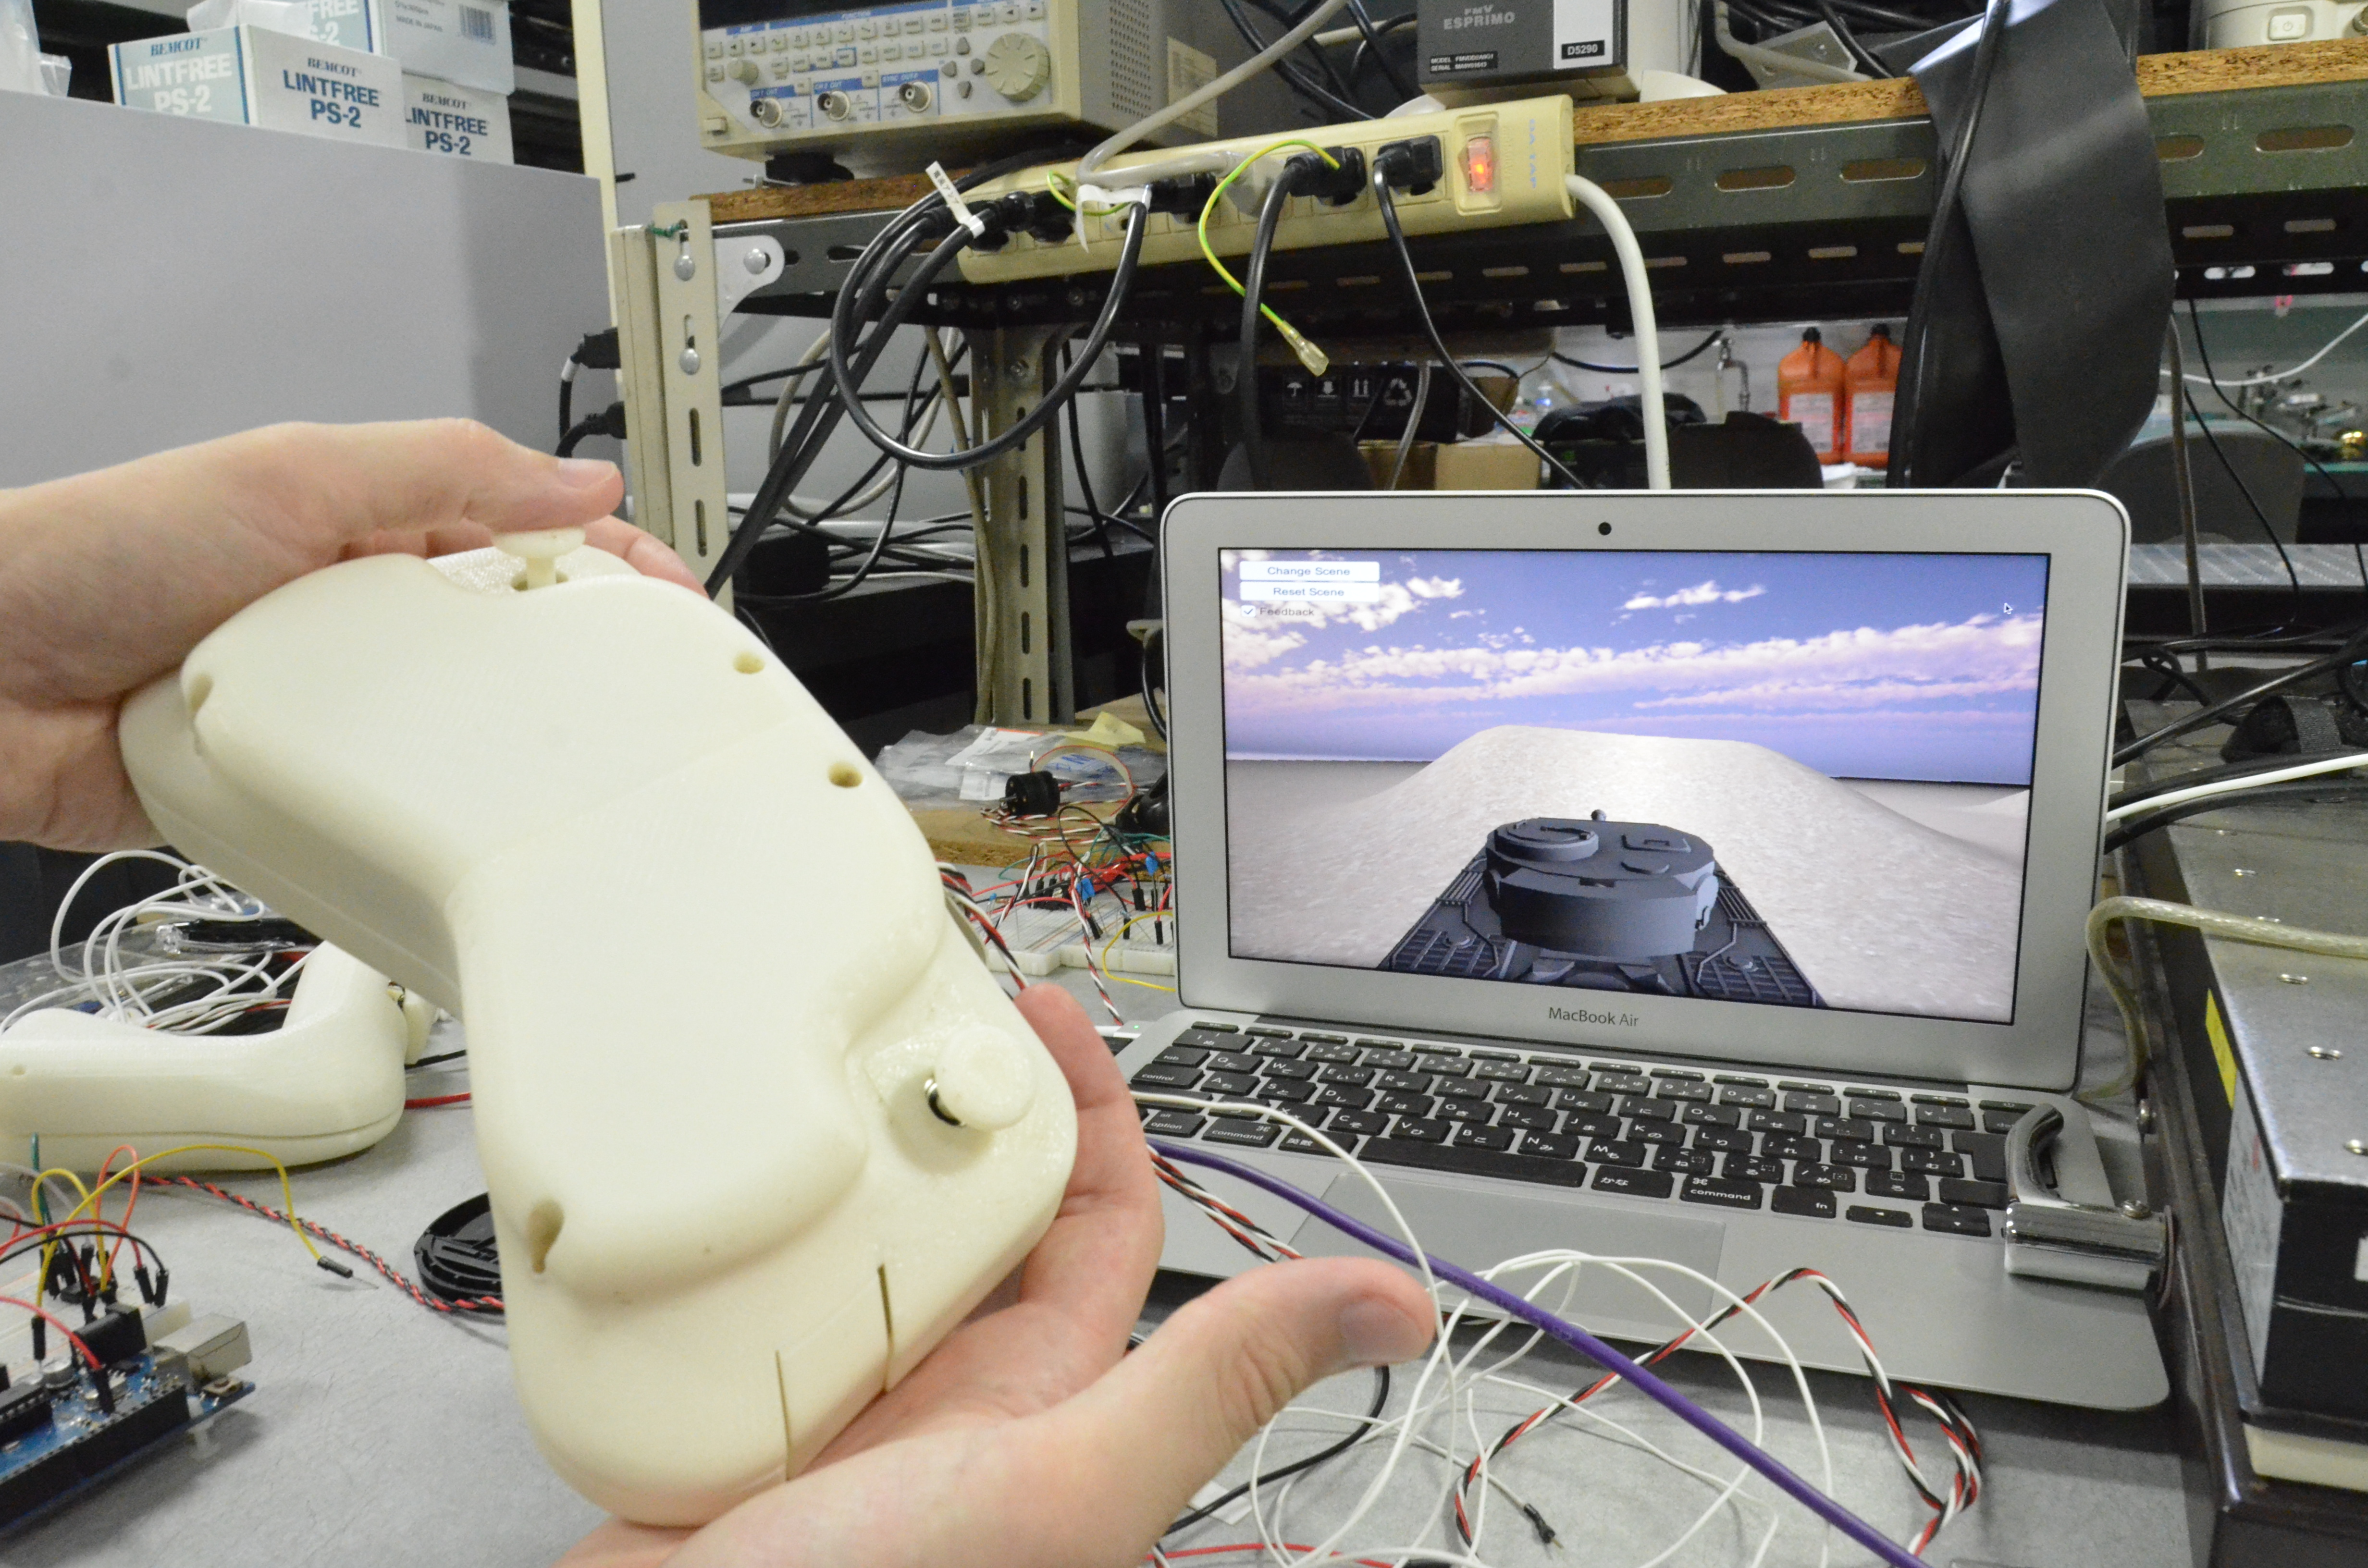
\includegraphics[width=0.6\linewidth]{Figs/unity_test_setup}
	\caption{Unity simulation test setup.}
	\label{fig:unity_test_setup}
\end{figure}
%TODO take picture to show test setup
For testing the controller in the simulated world, the Unity program from the previous research of this project has been used. With minor modifications of the control software, the controller could be tested with different feedback for the two stimulators. This time, only the combined roll-pitch feedback law has been used.\\
Since all communication delays have been eliminated, the simulated tank reacted instantly to the user's command and its orientation angles is fed back. \\
There is no latency feelable, neither when sending the commands, nor when receiving the feedback. The real-feel of the controller is better than before and even the maximum output force could be achieved when driving over the steep slopes of the environment. The range of the output force is appropriate for the desired feedback. And obstacles or slopes can be felt individually and intuitively on both sides.\\
This simulation only test shows that the latency reported in the previous section does not stem from the implementation of the series elastic actuators and justifies the choice of this actuation system.\\

\subsection{Overall Evaluation of the PlayStation Controller}
Overall one can say that the controller has achieved the performance requirements stated in the beginning of the project. \\ %TODO maybe reference here
The advantages of using SEA's are mostly the increased maximum output force and the decreased weight (VCM's tend to be very heavy due to the magnets). A drawback however is the size of the controller. The controller has been designed with several margins for dimensions and distances, leading to this bulky setup. If necessary, the design can be optimized in a future work, which would result in a much smaller controller than the current design.\\
Both control schemes (SEA and VCM) are straightforward and the output force can be controlled easily.\\
The disadvantages of the SEA implementation are the control speed and reaction time of the mechanical setup. As it has been shown in both testing environments, the mechanical response time is not the bottleneck in this setup.\\
Even though the maximum output force is enough to give a good feedback, it can be further increased. The motors that are used currently are not capable of compressing the springs to their maximal deflection. Therefore it is enough, to switch out the motors to have a higher torque. But when doing so, it should be verified, that the control speed of the motors do not affect the overall response time.\\
From the psychological points of view, the only shortcoming is the direction of the feedback which is application-specific. For this reason, and in order to write and test a parameter choice framework for future research projects, based on the current findings, a second controller has been designed.\\


\section{Design Framework}
This section provides a guideline for important design parameter choices, if one wants to design a similar haptic feedback controller based on series elastic actuators. It is mainly based on the findings from the PlayStation controller but also includes the main results of the second controller, called pilot controller. \\
Since the design framework depends on the target application, it is assumed to use the controller for robots similar to the Topy robot.

\subsection{Software and Control Choices}
In order to introduce no latency for control commands, it is important to have a high communication speed with no delay. In the current Arduino setup, one can decrease the command delay by using interrupts for the joystick commands. For immediate feedback, one can implement a feedforward control scheme that is fed from the joystick's positions directly to the stimulators.\\
The bottleneck of this setup was the fixed communication frequency of the Topy robot of maximum $5$ Hz. Due to the small changes of the feedback value, this operation frequency is still acceptable. But if one expects a highly fluctuating feedback, a higher communication frequency has to be opted for.\\
The suggested control scheme is a normal proportional controller, mainly due to the fact that it is bothersome to fine-tune the PID gains.\\
For haptic applications, it is suggested to have at least a motor control rate of $1$kHz which is the limit for the Arduino. If one opts for higher control frequencies, it is recommended to switch to an Mbed device or similar devices.
%software and control

\subsection{Mechanical Parameters}
One of the first mechanical design choices is the design of the controller itself. The PlayStation like controller has been chosen for consistency with the previous research, but also for the fact that most conventional controllers are based on this design. It is not required to copy this design, which is why a different approach has been chosen for the second controller design.\\
The feedback direction is target-application specific and results from the design. For the desired application, it is recommended to have a direct movement opposing force, as it is the case for the pilot controller design.\\
The weight only plays a minor role and any weight seems to be fine as long as the operator is comfortable with handling the controller.\\

The target point of contact with the user's palm is between the Mars and Venus region %TODO reference hand terminology
. This area is sensitive enough and can have a typical indentation of $5$mm which needs to be taken into account when calculating the necessary stroke of the stimulator. The palm pads' areas should be around $5$ to $10$ cm$^2$.\\

Another important element is the spring system that can be chosen. It is recommended to have a symmetric arrangement with springs of equal spring constant. Also, it should be paid attention to symmetries when assembling the springs, to assure a linear behavior when compressing. The length of the springs does not seem to be very important, as long as the compression is constrained to the perpendicular axis only. Testing different deflections has shown that the target stroke must be achievable and that it is better to have a margin if one wants to change the motors used to increase the output force.\\
The spring coefficients can vary and tests between $2$ and $24$ N/mm have shown promising results. %TODO emphasize these tests or outcome, and reference somehow, link to results or data

The motors greatly influence the performance of the controller. The reduction ratio should be high enough to guarantee the target output force, while assuring the desired control speed. The target output torque can be used to calculate the output force approximately. But one should keep in mind that some energy is lost in friction and efficiency of the motor and gear assembly.
%mechanical (springs (length, size, arrangement), motors (speed/reduction, output torque), design (orientation, stimulators, etc.), weight)

\subsection{Electrical Parameters}
The electric components that have been used are mainly the potentiometer for the joysticks and the photoreceptors for distance sensing.\\
The photoreceptors have very different characteristics and all thresholds need to be identified individually. Furthermore, the output function is not linear for a big range of distances and the sensitivity also depends on the distance. If a high performance is expected from the controller, it is recommended to find a different solution or a better performing sensor.\\
Furthermore, it is recommended to filter the motor commands to convert the Arduino output PWM to a more steady voltage level, to protect the amplifiers from overfitting the signal.\\
Also, it was necessary to have a voltage follower (a simple operational amplifier with unitary gain) in order to reduce interfering effects on the distance sensors.
%electrical (sensors, joystick)

%say what parameters are important, how they affect the controllers, etc.
%say what i have found for my PS controller and what i can change

\section{Pilot Controller}
Based on the framework from the previous section, a new controller has been devised, mainly focusing on a different design and on a more optimal feedback direction.

\subsection{Working Principle (cam)}%TODO put text from april here
Has already been stated in April's monthly report.

\subsection{Design and Parameters}
When designing this controller, the design of an airplane yoke has been used as a model. Therefore it is from now on called pilot controller. In order to have a nice fit to the palms, the circumference has been chosen to be close to the airplane yokes or conventional car steering wheels. The joysticks' position is such that the stimulator touches the same area of the palm as in the previous controller and research (Venus and Mars area of the hand). This time the feedback direction is perpendicular towards the user, which ensures a more intuitive feeling for the desired application.\\
The most important parameters in this system are the length of the lever and the springs. For the prototype, the levers length has been fixed to roughly $100$ mm and a set of four springs with $1$ N/mm each have been used. Their length is $10$ mm and they have an allowable deflection ratio of $40$\%.\\
The stimulators area is kept almost the same with $7.5$ cm$^2$.\\
The motors play an important role again and for this design, the motors with the reduction gear of $33:1$ have been implemented.

When designing the rotational cam part, a spiral-like freeform has been drawn to keep the angle-to-distance ratio as linear as possible. The operational range of the motor shaft is $110 ^\circ$. It is, the full stroke of the lever can be achieved by rotating the motor shaft and the attached rotation cam by this angle.\\

The operational distance for the photoreceptors is between $11$ mm and $8$ mm. 
Again the operational range of the photoreceptors can be identified.

\begin{figure}[h!]
	\centering
	\begin{tabular}{|l|c|c|c|c|c|}
		\hline
		& Sensor reading & Distance & Sensor reading & Distance & Max output  \\
		& MAX (rest) & (rest) & MIN (compression) & (compression) & force \\ \hline \hline
		Left side & 800 & 11mm & 550 & 8mm & 12N \\ \hline
		%Right side & 870 &2.2mm & 700 & 8mm & 10.8N \\ \hline
	\end{tabular}
	\caption{Identified operational range for the photoreceptors in the pilot controller.}
	\label{tab:oper_range_pilot}
\end{figure}
%state the parameter choices that i have made based on previous findings
\subsection{advantages and disadvantages}%TODO is this really necessary or can i write it under design and parameters
%state advantages and disadvantages
\subsection{Analytical results}
%state analytical results (if available)
\subsection{Frequency Response Analysis}
Similar to the previous frequency response analysis, the controller has been tested when feeding a sine wave in the range of $1$ Hz up to $100$ Hz. The result for the P-controlled device can be seen in figure \ref{fig:pilot_bode_P02}

\begin{figure}[h!]
	\centering
	\includegraphics[width=0.6\linewidth]{Figs/pilot_bode_P02}
	\caption{Frequency response function of the P-controlled pilot controller.}
	\label{fig:pilot_bode_P02}
\end{figure}

The bode diagram resembles the one of the previous setup, with the main difference, that it seems to be shifted towards lower frequencies. The phase offset changes almost linearly from $45 ^\circ$ to $200 ^\circ$. Analogously, it is argued that the initial phase lag for low frequencies stems from the different filters that have been implemented in the same manner. Regarding the magnitude plot however, it is important to note that the resonance frequency is much lower, namely $4$ Hz.\\

In the current design of the pilot controller, the lever is roughly $100$ mm and has been fabricated using an $8$ mm thick poly-acetal plate. Due to the relative low thickness, the lever can deform and thus leads to an additional spring element in the system. Furthermore, the rotation cam is not coupled to the lever and thus cannot make pull it back in order to decrease the springs' compression, even if a negative voltage is applied. This leads to a lower overall performance and results in a lower resonance frequency.\\
In order to deal with this issue, it is recommended to preload the lever that pulls it back faster than normal, or couple the rotational cam with the lever.

\subsection{Pilot-Controller Testing}
%state real feel, latency, transparency and stability
\subsection{Outlook}
%state possible improvements for future work


\section{Discussion}	

\section{Conclusion}


\section{Outlook}



	
	%�����܂�
}


